\documentclass[onecolumn]{article}

%\usepackage{aistats2024}
% If your paper is accepted, change the options for the package
% aistats2024 as follows:
%
\usepackage[preprint]{neurips_2023}
\RequirePackage{amsthm,amsmath,amsfonts,amssymb}
\RequirePackage{titletoc}
\RequirePackage{graphicx}
% \usepackage{subfigure}
\usepackage{subcaption}
\usepackage{appendix}
\usepackage[utf8]{inputenc} % allow utf-8 input
\usepackage[T1]{fontenc}    % use 8-bit T1 fonts
\usepackage[switch, modulo]{lineno}
%\linenumbers
\usepackage{url}            % simple URL typesetting
\usepackage{booktabs}       % professional-quality tables
\usepackage{nicefrac}       % compact symbols for 1/2, etc.
\usepackage{microtype}      % microtypography
\usepackage{algpseudocode}
\usepackage{algorithm}
\usepackage{dsfont}
\usepackage{mathtools}
\usepackage{bm}
\usepackage{mathrsfs}
\usepackage[colorlinks=true,citecolor=blue]{hyperref}

\usepackage[textsize=tiny,textwidth=20mm]{todonotes}  % TODO remove this later

\author{%
  Mahmoud Hegazy \\
  IP-Paris\\
  mahmoud.hegazy@ip-paris.fr
  \And
  Inès Vati \\
  MVA ENS Paris-Saclay \\
  ines.vati@eleves.enpc.fr\\
}
\title{Medical Image Analysis Project}
\usepackage{colortbl}
\definecolor{lightgray}{rgb}{0.9,0.9,0.9}
\definecolor{lightred}{rgb}{1,0.8,0.8}
\definecolor{lightgreen}{rgb}{0.6,1,0.6}
\definecolor{lightyellow}{rgb}{1,1,0.5}
\definecolor{lightgrey}{rgb}{0.8,0.8,0.8}

\newcommand{\prob}{\mathbb{P}}
\newcommand{\esp}{\mathbb{E}}
\newcommand{\ehat}{\hat{\mathbb{E}}}
\newcommand{\K}{\mathbb{K}}
\newcommand{\ccal}{{\cal C}}
\newcommand{\scal}{{\cal S}}
\newcommand{\rcal}{{\cal R}}
\newcommand{\ical}{{\cal I}}
\newcommand{\mcal}{{\cal M}}
\newcommand{\bcal}{{\cal B}}
\newcommand{\ocal}{{\cal O}}
\newcommand{\xcal}{{\cal X}}
\newcommand{\dcal}{{\mathscr D}}
\newcommand{\fcal}{{\cal F}}
\newcommand{\ncal}{{\cal N}}
\newcommand{\hcal}{{\cal H}}
\newcommand{\acal}{{\cal A}}
\newcommand{\pcal}{\mathbb{P}}
\newcommand{\qcal}{\mathcal{Q}}
\newcommand{\vcal}{{\cal V}}
\newcommand{\ecal}{{\mathscr E}}
\newcommand{\ccalinf}{{\cal C}^\infty}
\newcommand{\btheta}{\boldsymbol{\theta}}
\newcommand{\beps}{\boldsymbol{\varepsilon}}
\newcommand{\mbe}{\mathbf{e}}
\newcommand{\beq}{\begin{equation}}
\newcommand{\eeq}{\end{equation}}
\newcommand{\erf}{\text{erf}}
\newcommand{\mb}{\mathbf}
\newcommand{\one}{\mathbf{1}}
\newcommand{\rep}[1]{\begin{normalize}
\fbox{
\begin{minipage}{\textwidth} #1 \end{minipage}}\end{normalize}}
\def\rset{\mathbb{R}}
\def\cset{\mathbb{C}}
\def\zset{\mathbb{Z}}
\def\nset{\mathbb{N}}
\def\mcf{\mathcal{F}}
%\def\argmax{\mathop{\rm arg\, max}}
%\def\argmin{\mathop{\rm arg\, min}}
\newcommand{\ih}{h}
\newcommand{\ihp}{g}
\newcommand*{\mhegz}[1]{\textbf{\textcolor{blue}{#1}}}
\newcommand*{\ivat}[1]{\textbf{\textcolor{orange}{#1}}}
\newcommand{\QD}{AINQ}
\newcommand{\floor}[1]{\left \lfloor #1 \right \rfloor }
\newcommand{\ceil}[1]{\left \lceil #1 \right \rceil }
\newcommand{\norm}[1]{\left \lVert #1 \right \rVert}
\newcommand{\open}[1]{\left ( #1 \right )}
\newcommand{\closed}[1]{\left [#1 \right]}
\newcommand{\ens}[1]{\left \{ #1 \right \} }
\newcommand{\modu}[1]{\left \lvert #1 \right \rvert }
\newcommand\inner[2]{\left \langle #1, #2 \right \rangle}
\DeclareMathOperator{\expec}{\mathbb{E}}

\definecolor{britishracinggreen}{rgb}{0.0, 0.26, 0.15}
\newcommand{\xcross}{\textcolor{red}{$\times$}}
\newcommand{\greenV}{\textcolor{britishracinggreen}{$\checkmark$}}

\newcommand{\DP}{\text{DP}}
\newcommand{\LDP}{\text{LDP}}
\newcommand{\eps}{\varepsilon}
\newcommand{\lcal}{\mathcal{L}}

\newcommand{\bo}{\mathcal{O}}

\newcommand\tab[1][1cm]{\hspace*{#1}}
\newcommand{\Uni}{\mathcal{U}}
\newcommand{\diff}{\mathrm{d}}

\newtheorem{theorem}{Theorem}
\newtheorem{corollary}{Corollary}
\newtheorem{definition}{Definition}
\newtheorem{lemma}{Lemma}
\newtheorem{remark}{Remark}
\newtheorem{example}{Example}
\newtheorem{proposition}{Proposition}
\newtheorem{Conjecture}{Conjecture}
\newtheorem{assumption}{Assumption}
%%%%%%%%%%%%%%%%%%%%%%%%%%%%%%%%%%%%%%%%%%%%%%%%%%%%%%%%%%%%%%%%%%
\DeclareMathOperator{\var}{\mathbb{V}}
\DeclareMathOperator{\spann}{Span}
\DeclareMathOperator{\ent}{\mathcal{H}}
\DeclareMathOperator{\diffent}{h}
\newcommand{\1}{\mathds{1}}

\DeclareMathOperator{\supp}{Supp}
\DeclareMathOperator{\conv}{Conv}
\DeclareMathOperator{\tr}{Tr}
\DeclareMathOperator{\image}{Im}
\DeclareMathOperator{\kernel}{Ker}
\DeclareMathOperator{\diag}{diag}
\DeclareMathOperator{\sgn}{sgn}
\DeclareMathOperator{\rk}{rank}
\DeclareMathOperator{\relu}{\texttt{ReLU}}
\DeclareMathOperator{\op}{Op}
\DeclareMathOperator{\vect}{vec}
\DeclareMathOperator{\MSE}{MSE}
\DeclareMathOperator{\argmax}{argmax}
\DeclareMathOperator{\argmin}{argmin}
\DeclareMathOperator{\unif}{Unif}
\newcommand{\pr}[1]{\left({#1}\right)}

\begin{document}

\maketitle
\section{Introduction} 
\textit{Inès Vati} and \textit{Mahmoud Hegazy} 

In the area of Convolution Neural Network (CNN) based segmentation, widely employed loss functions, such as Dice or cross-entropy, have been instrumental in delineating segmentation regions. However, a critical drawback emerges when tackling highly unbalanced segmentation. As regions are highly uneven, the values obtained from regional summations vary drastically across classes, spanning several orders of magnitude. This inherent imbalance poses a substantial challenge to training performance and stability.


% we dnote $X_{i,\cdot}$ the $i$-th row, $X_{\cdot, j}$ the $j$-th column, and $X_{ij}$ the component in the $i$-th row and the $j$-th column.  

% \textbf{Quick Summary:} We consider the problem of regimentation over 2 classes, labels by $\ens{0,1}$. We generally consider performing segmentation using a neural network parameterized by $\theta$. For an image $X\in \rset $ let $g:\rset^d \rightarrow \ens{0,1}^d$ be the ground-truth i.e. $g(X)_i=1$ if $X_i$ is in class $0$. Designing a loss function for a segmentation task can be tackles in a number of way. For simplicity, define $S_\theta(X) = f_\theta(X)_{\cdot, 1}$ i.e. for an image $X$, $S_\theta(X)$ is the softmax probability that a pixel/voxel belongs to class $1$. We list below the definition of some losses. 
% \ivat{I think we should not put the definition of the loss in the intro. We can discuss it in the next meeting}
% \subsection{Cross entropy loss:} 
% \begin{equation}
% \begin{split}
%     \lcal_{CE}(X, \theta) = -\inner{g(X)}{\log(c_\theta(X))} -  \inner{\one-g(X)}{\log(\one-c_\theta(X))}
% \end{split}
% \end{equation}
% where $\log$ is taken element-wise.It measures the affinity between predicted regions $c_\theta(X)$  and the ground-truth regions $g(X)$. However, it assumes identical distribution of all the samples and classes (including background/foreground). Therefore, using it alone is not well-suited for unbalanced segmentation class problems.
% \subsection{Generalized Dice Loss:} 
% \begin{equation}
% \begin{split}
%         \lcal(X, \theta) = 1-2 \frac{w_1\inner{g(X)}{c_\theta(X)}+w_0\inner{\one-g(X)}{\one-c_\theta(X)}}{w_1\inner{c_\theta(X)+g_\theta(x)}{\one}+w_0\inner{2-c_\theta(X)-g(X)}{\one}}    
% \end{split}
% \end{equation}
%     where $w_0=\norm{1-g(X)}_F^{-2}$ and $w_1 =\norm{g(X)}_F^{-2}$


To address this issue, \citet{kervadec_boundary_2021} propose a boundary-based loss function in their article. Departing from conventional methodologies, this loss function operates on the space of contours rather than regions. The key advantage lies in its ability to mitigate the difficulty of highly unbalanced regions by penalising mistakes proportionally to the distance between the mistake and the interfaces of regions. This circumvents the pitfalls of unbalanced sums over the regions themselves. Moreover, boundary loss not only addresses imbalance issues but also complements regional information and can be seamlessly integrated with standard regional loss. In addition, it can be implemented with any existing deep network architecture designed for segmentation. 

From this perspective, this article introduces the paradigm of boundary-based loss functions for CNN segmentation. We now first introduce the mathematical and notational framework needed to proceed with defining boundary loss. Then, we proceed to discuss other segmentation loss functions and some of the related work. Finally, we will evaluate the method on two different datasets, each presenting a unique set of difficulties. 
% We use $\rset^{m\times n}$ to denote $\rset^m \times \rset^n$. For $X\in \rset^{m\times n}$, we dnote $X_{i,\cdot}$ the $i$-th row, $X_{\cdot, j}$ the $j$-th column, and $X_{ij}$ the component in the $i$-th row and the $j$-th column. 

% We noTo define the boundary loss we define the boundary loss 
% For simplicity we will consider $k=2$ i.e. there are two segmentation classes such as. For the an image $X\in \rset$, we denote the the ground truth by $g$

\textbf{Problem Statement:} We consider a  segmentation function $f_\theta$ parameterized by $\theta$ such that  $f_\theta: \rset^s \times \rset^c \rightarrow \rset^s \times \Delta^{k-1}$ taking in an image and outputting softmax probabilities over $k$ classes. Here, $s$ represents the dimension of the underlying images. Using $\rset^{m\times n}$ to denote $\rset^m \times \rset^n$, and with the slight abuse of notation, $s$ can be taken as a placeholder for $h\times w$ for 2D or $h\times w\times d$ for 3D tensors.  $c$ represents the channel (3 for RGB, 2 for MRI, 1 for grayscale) and $\Delta^{k-1}\subset \rset^k$ is the standard simplex.

In addition, let $\inner{\cdot}{\cdot}$ be the standard inner product, $\|\cdot\|_F$ the Frobenius norm, $\bm{a}$ be the all vector/matrix/tensor in $\rset^d$ of repeated $a$. For $X\in \rset^{m\times n\times p}$, $X_i$ is the component at index $i \in [m]\times [n] \times [p]$


For notational simplicity, we restrict our attention to the case where $k=2$ for most of this report. The extension of the boundary loss to multiclass segmentation will be later introduced in section \ref{sec:multiclass}. For an image $X$, we denote the ground truth by  $g:\rset^d \rightarrow \ens{0,1}^d$ such that $g(X)_i=1$ if $X_i$ is in class $1$. Also define $c_\theta(X) = f_\theta(X)_{\cdot, 1}$ i.e. for an image $X$, $c_\theta(X)$ is the softmax probability that a pixel/voxel belongs to class $1$. 

\textbf{A note on notation:} The original article opted mostly for integral-based notation to motivate and define the boundary loss function. We found that it obscured the computational ease of this loss. Thus, we opted for a more vectorised notation, where most operations are written as matrix products and element-wise operations, that are extremely ubiquitous, fast, and scalable in modern scientific computing. 

\section{Boundary Loss} 
\textit{Mahmoud Hegazy} 


At its core, boundary loss is an approach of penalizing mistakes w.r.t to their distance from the boundary between two regions. In practice, this reduces to a voxel-wise multiplication between the network predictions and a pre-computed distance map.

To define the boundary loss, we first introduce the necessary sets and notation. Let $I$ be the set of all indices of an image $X$. Then, define $G_0(X) \coloneqq \ens{i | g(X)_i = 0}$, $G_1(X)\coloneqq I / G_0(X)$, $C_0(X) \coloneqq \ens{i| c_\theta(X)_i\leq\alpha}$, and $C_1(X) = I/C_0(X)$ where $\alpha$ is a hyperparameter by the user (typically $1/2$). Define the boundary set $\partial G(X) \coloneqq \ens{d \in G_1(X) | N(d)\cap G_0(X)\neq \emptyset}$, where $N(d)$ are the neighbouring indices to $d$. 

Using the boundary set $\partial G$, it is now possible to define a distance between any point and $\partial G$. For example, consider a 3D image of width $w$, height $h$, and depth $d$ voxels. Then, $I = [w]\times [h]\times [d]$ and for any $x, y\in I$ we can define a Euclidean-like distance on the grid 
\begin{equation}
    (x,y) = \sqrt{\alpha_1^2(x_1-y_1)^2+\alpha_2^2(x_2-y_2)^2+\alpha_3^2(x_3-y_3)^2},
\end{equation}
with $\alpha_1$, $\alpha_2$, and $\alpha_3$ representing sampling constants i.e. estimations on how far two voxels are in real life. We can now define the projection onto $\partial G$ and a corresponding distance using $d$ w.r.t to the index as follows

\begin{gather}
    \Pi_{\partial G(X)}(i) \coloneqq \argmin_{j \in \partial G(X)} d(i,j)
\end{gather}

Dropping the notational dependence on $X$, we now define the distance-map function $\phi:\rset^d\rightarrow \rset^d$ as 
\begin{equation}
\label{eq:boundary_distance}
\phi(X)_i=
\begin{cases}
& -d(i,\Pi_{\partial G}(i) )\;\;  \text{for} \; i \in G(X) \\
& d(i,\Pi_{\partial G}(i) ) \;\;\text{otherwise}
\end{cases} .\text{}
\end{equation}

 \begin{figure}[h!]
    \centering
     \begin{subfigure}{0.49\textwidth}
         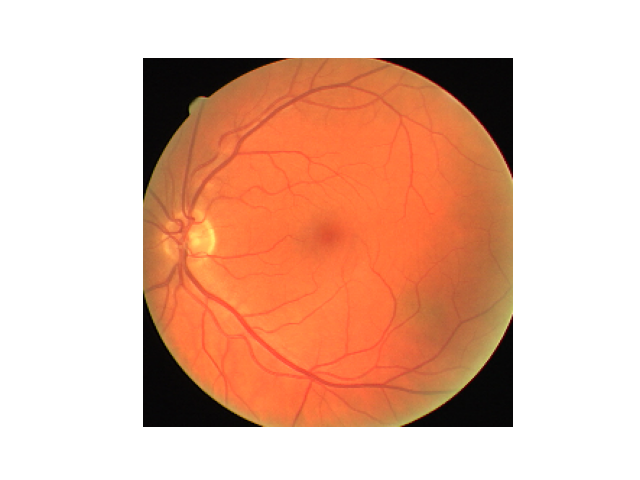
\includegraphics[width=\textwidth]{figures/ex_dist1.png}
         \caption{RGB Input Image}
     \end{subfigure}
     \hfill
     \begin{subfigure}{0.49\textwidth}
     \centering
         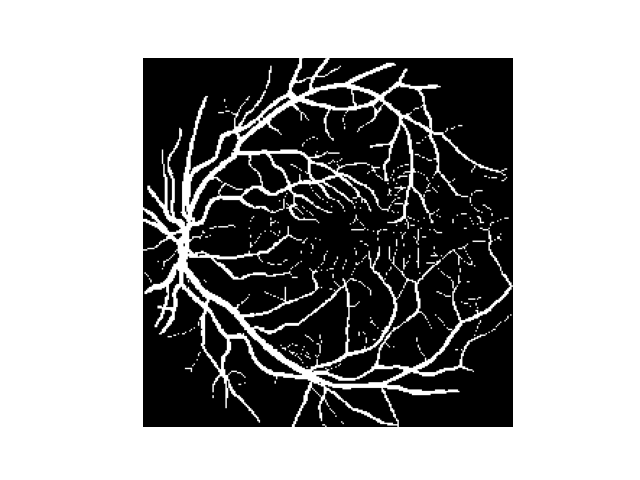
\includegraphics[width=\textwidth]{figures/ex_dist2.png}
         \caption{Segmentation map}
     \end{subfigure}
     \begin{subfigure}{0.44\textwidth}
     
         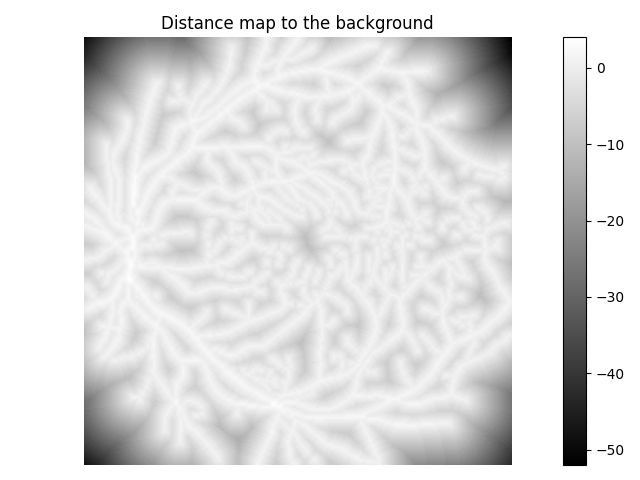
\includegraphics[width=\textwidth]{figures/ex_dist3.png}
         \caption{Distance map to $G_0$}
     \end{subfigure}
     \hfill
     \begin{subfigure}{0.44\textwidth}
     \centering
         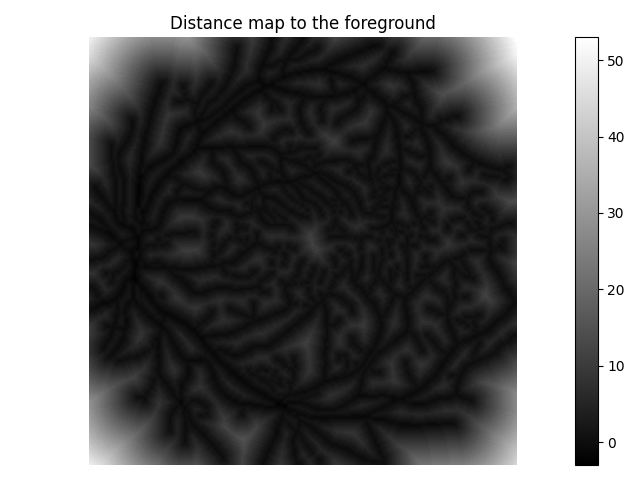
\includegraphics[width=\textwidth]{figures/ex_dist4.png}
         \caption{Distance map to $G_1$}
     \end{subfigure}
     \caption{Illustration of distance map on DRIVE Dataset} $G_1$ corresponds to the set of pixels constituting the vessels.
     \label{fig:dist_map_DRIVE}
 \end{figure}
To illustrate the distance map, we refer to figure \ref{fig:dist_map_DRIVE}. Finally, the boundary distance can be written as 
\begin{equation}
    \lcal_B(X, \theta) \coloneqq \inner{c_\theta(X)}{\phi(X)}.
\end{equation}
First, we note the above formulation of $\phi$ was extracted from the source code. The statement in the paper is more general and leaves some freedom for its implementation. In essence, for a voxel $i$ in $G(X)$, this definition of the boundary loss penalizes any prediction probability of a voxel being outside the boundary. Furthermore, the penalty is scaled the more inside the $G(X)$ lies. Interestingly, in contrast to most common loss functions, the boundary can and will often be negative in training. However, the function remains bounded below and will work out of the box with any first-order solver optimizing $\theta$.

For an $N$-class segmentation problem, applying boundary loss can be achieved by transforming the problem to a set of $N$ one-vs-all binary segmentation problems. Let $\lcal^i_\bcal$ be the loss associated with the $i$-th problem, then the boundary loss of the $N$-class problem can be written as $\lcal_\bcal(X, \theta)=\sum_{i=1}^N \lcal^i_\bcal(X,\theta)$
\label{sec:multiclass}

% \begin{itemize}
%     \item \textbf{Cross entropy loss:} \begin{equation}
%     \lcal_{CE}(X, \theta) = -\inner{g(X)}{\log(c_\theta(X))} - \inner{\one-g(X)}{\log(\one-c_\theta(X))}
%     \end{equation}
%     where $\log$ is take element-wise.

%     It measures the affinity between predicted regions $c_\theta(X)$  and the ground-truth regions $g(X)$. However, it assumes identical distribution of all the samples and classes (including background/foreground). Therefore, using it alone is not well-suited for unbalanced segmentation class problems.

%     \item \textbf{Generalized Dice Loss:} \begin{equation}
%         \lcal(X, \theta) = 1-2 \frac{w_1\inner{g(X)}{c_\theta(X)}+w_0\inner{\one-g(X)}{\one-c_\theta(X)}}{w_1\inner{c_\theta(X)+g_\theta(x)}{\one}+w_0\inner{2-c_\theta(X)-g(X)}{\one}}
%     \end{equation}
%     where $w_0=\norm{1-g(X)}_F^{-2}$ and $w_1 =\norm{g(X)}_F^{-2}$
% \end{itemize}



% \section{The proposed method}
% \ivat{You can add what you wrote on your "quick notes" here about the definition of the boundary loss + slight explanation why is it more interesting} \\ 

% The boundary loss, at its core, is a pixel-wise multiplication between the network predictions, and a pre-computed distance map.


\section{Related work, Impact and Discussion} \textit{Ines Vati}

The cross-entropy loss is one of the most common loss functions for classification tasks. In particular, segmentation can be regarded as a voxel-wise classification problem. Under this setting, the cross-entropy loss is defined as

\begin{equation}\label{eq:CE}
\begin{split}
    \lcal_{CE}(X, \theta) = -\inner{g(X)}{\log(c_\theta(X))} -  \inner{\one-g(X)}{\log(\one-c_\theta(X))},
\end{split}
\end{equation}

where the $\log$ is taken element-wise. It measures the affinity between predicted regions $c_\theta(X)$ and the ground-truth regions $g(X)$. However, it assumes identical distribution of all the samples and classes (including background/foreground). Therefore, using it alone is not well-suited for unbalanced segmentation class problems.

Several studies have already been conducted to address the challenges posed by the unbalanced region sizes in medical images. \cite{sudre_generalised_2017} generalized the Dice loss by weighting according to the squared inverse of class-label frequency, denoted as $w_0$ and $w_1$.
This approach was shown to outperform the cross-entropy loss. The generalized Dice loss (GDL) is defined as 
 \begin{equation}\label{eq:GDL}
        \lcal_{GDL}(X, \theta) = 1-2 \frac{w_1\inner{g(X)}{c_\theta(X)}+w_0\inner{\one-g(X)}{\one-c_\theta(X)}}{w_1\inner{c_\theta(X)+g_\theta(x)}{\one}+w_0\inner{2-c_\theta(X)-g(X)}{\one}},
    \end{equation}
with $w_0=\norm{1-g(X)}_F^{-2}$ and $w_1 =\norm{g(X)}_F^{-2}$.


However, Dice losses could still face challenges when addressing very small structures. In highly unbalanced scenarios, misclassification of pixels might result in loss reductions, leading to unstable optimization. Another reason that may explain the poor performances of Dice losses when dealing with extreme foreground/background class imbalance is that the Dice similarity coefficient (DSC)\footnote{Note that Dice loss is 1 - DSC.} corresponds to the harmonic mean between precision and recall. Indeed, using the same notation as above, we recover:
\begin{align*}
    DSC &= \frac{2 |C_1 \cap G_1|}{|C_1| + |G_1|} = \frac{2}{\frac{|C_1|}{|C_1\cap G_1|} + \frac{|G_1|}{|C_1 \cap G_1|}}\\
    &= \frac{2}{\frac{TP + FP}{TP} + \frac{TP + FN}{TP}} \\
\end{align*}

Recognizing the precision and recall, it can be written as the following harmonic mean
\begin{align*}
    DSC &= \frac{2}{\frac{1}{\text{Precision}} + \frac{1}{\text{Recall}}} \\
    &= \frac{2}{2 + \frac{FP}{TP} + \frac{FN}{TP}}.
\end{align*}
When the true positives remain the same, one notices that false positives and false negatives are equally important, making this loss inappropriate when both types of errors are not equally high (in particular when $FP >> FN$). Indeed, easily classified negatives comprise the majority of the loss and dominate the gradient. \cite{lin_focal_2018} proposed to reshape the cross-entropy loss function to down-weight "easy" examples and thus focus on hard negatives. The focal loss is defined as 
\begin{equation}
    \lcal_{FL}(X, \theta) = -\inner{g(X)}{\open{1 - c_\theta(X)}^\gamma \log(c_\theta(X)} - \inner{1-g(X)}{c_\theta(X)^\gamma \log(1-c_\theta(X))}
\end{equation}
with $\gamma \geq 0$ a tunable \textit{focusing} parameter.
It implies that when the predicted probability $c_\theta(X)_i$ of pixel $i$ to belong to $C_1$ is small, its values have a higher weight in the loss function. 

Furthermore, since 2019-2020, incorporating the distance transform maps of image segmentation labels into CNN pipelines, has received significant attention. For example, \cite{ma_how_2020} benchmarked five methods using the signed distance map. In addition to the method studied in this report, they have evaluated two other loss functions: the Hausdorff distance loss (\cite{karimi_reducing_2019}) and the signed distance map regression loss (\cite{xue_shape-aware_2019}). They run 70 experiments to tune each method to achieve the best performance. According to their experimental results, all three losses have the potential to improve the performance of baseline CNNs. However, they observed that the performance gains are not consistent in different datasets and highly depend on implementation details like learning rates, loss functions and so on. 

Nonetheless, several works still rely on the proposed boundary loss. For instance, \cite{ribalta_lorenzo_multi-modal_2020} studied multi-modal U-Net-based architecture with unsupervised pre-training and surface loss components for brain tumour segmentation which allowed them to seamlessly benefit from all magnetic resonance modalities during the delineation.  

The result presented in (\cite{kervadec_boundary_2021}) shows that the proposed boundary loss does not work alone. It becomes interesting when it is associated with another regional loss $(\lcal_{R})$ with a certain weight. They specified that a suitable loss would be
\begin{equation}
    \lcal = \lcal_{R} + \alpha\lcal_{B}
\end{equation}
with $\alpha\in\mathbb{R}_+$ a parameter balancing the two losses. The chosen regional loss would be one of the above like the cross-entropy loss or the generalized Dice loss.


\section{Experiments}
For the experimental settings, we considered two datasets each representing a challenging setting. First, we considered the ACDC dataset \citep{bernard2018deep}, which is a multi-class segmentation dataset for heart delineation (left ventricle, right ventricle, myocardium, and background). In addition, we considered the DRIVE dataset \citep{staal2004ridge}, which is a binary segmentation dataset for retinal vessel extraction.


\subsection{ACDC Dataset}
\textit{Mahmoud Hegazy}


The ACDC dataset consists of 3D heart MRI scans of 150 people with 100 reserved for training and 50 for validation. Ground truth manual segmentation is available for all participants. The 3D scans are sliced into a sequence of 2D scans to reduce the computational cost.  For our implementation, we relied on the source code provided by the authors\footnote{https://github.com/LIVIAETS/boundary-loss}. In particular, we were interested in this dataset for two reasons. The first is that it tests the ability of the boundary loss to scale to multi-class problems. In addition, the performance on this dataset was not reported in the article \cite{kervadec_boundary_2021}. Sadly without access to a dedicated GPU, the computational cost of this experiment is high and we could conduct the experiments on the boundary loss without exploring other benchmarks.

For the experimental setting, we used E-Net \cite{paszke2016enet} architecture. As an optimization algorithms, we used Adam \cite{kingma2014adam} with learning rate $5\times10^{-3}$, $\beta_1=0.9$, $\beta_2=0.99$, and a batch size of $8$. During the training, we also measure the Dice loss \eqref{eq:GDL} to evaluate the relation between minimizing the boundary loss and the performance w.r.t the Dice loss. 

We report the results of the ACDC experiments in figures \ref{fig:plot1} and \ref{fig:plot2}. Figure \ref{fig:plot1} displays the boundary loss scaled to $0,1$ and the dice loss recorded during training. On the training set, minimizing the boundary loss strongly corresponded to smaller values of the Dice loss. However, on the validation set, the Dice loss fluctuated and such a strong relation was not observed. It is not immediately clear to us the reason behind such disparity. We believe that it is due to mistakes committed around the contour regions, as such mistakes are more penalized under the Dice loss. At the same time, such mistakes can be avoided on the training set due to overfitting. Figure \ref{fig:plot2} illustrates the output of the segmentation function over the validation set.
\begin{figure}[h!]
    \centering
    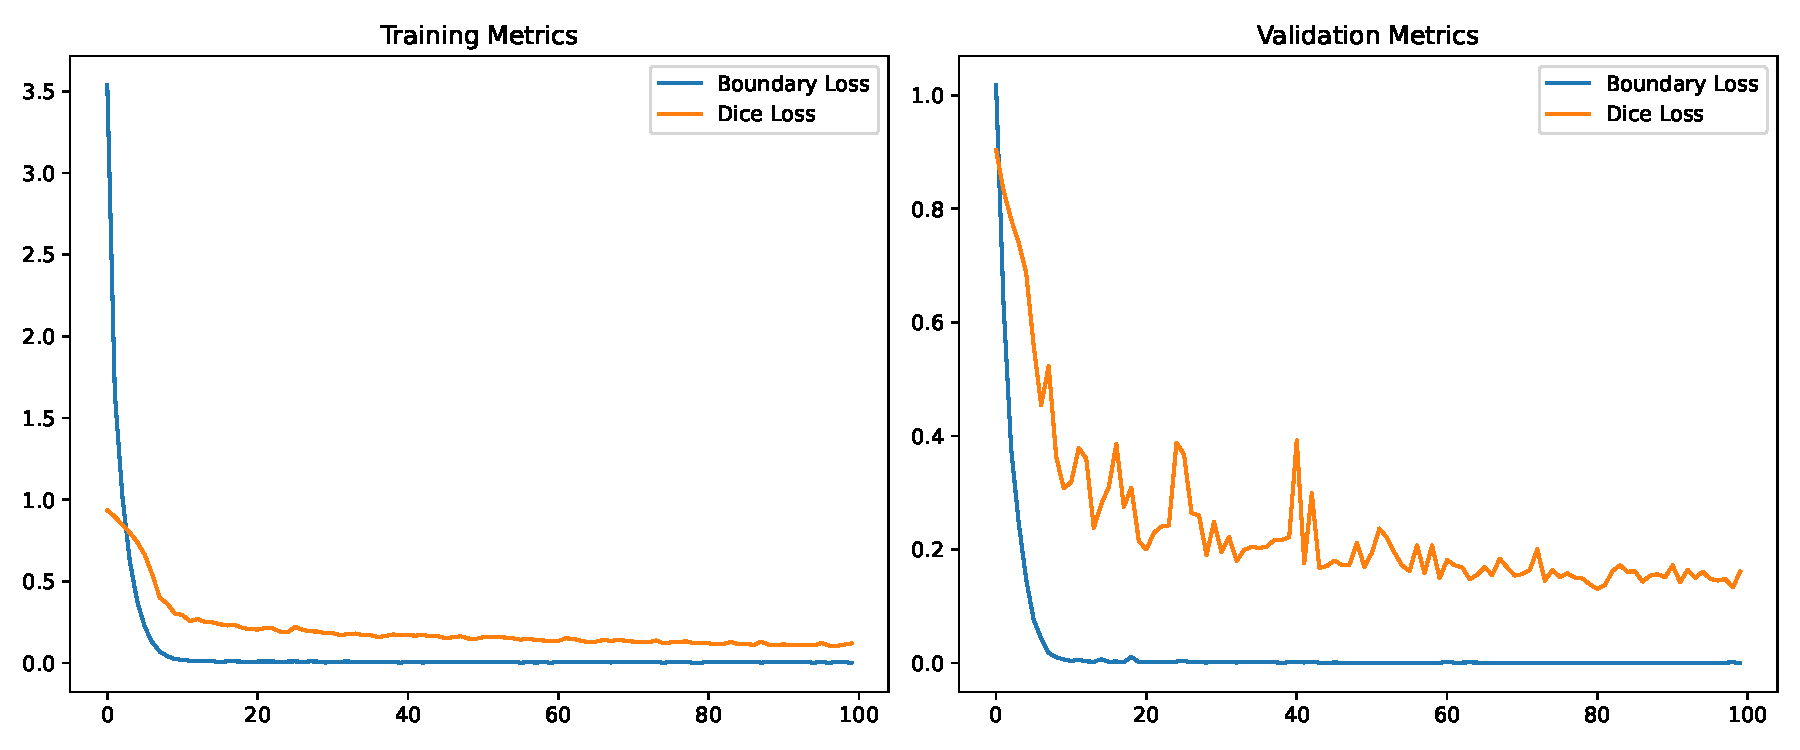
\includegraphics[width=0.8\linewidth]{figures/plot1.pdf}
    \caption{Boundary loss and Dice loss on the training and validation sets of ACDC dataset. As the boundary loss on ACDC is negative and on a different scale, the boundary loss was called to $(0,1)$ for visual comparison}
    \label{fig:plot1}
\end{figure}
\begin{figure}[H]
    \centering
    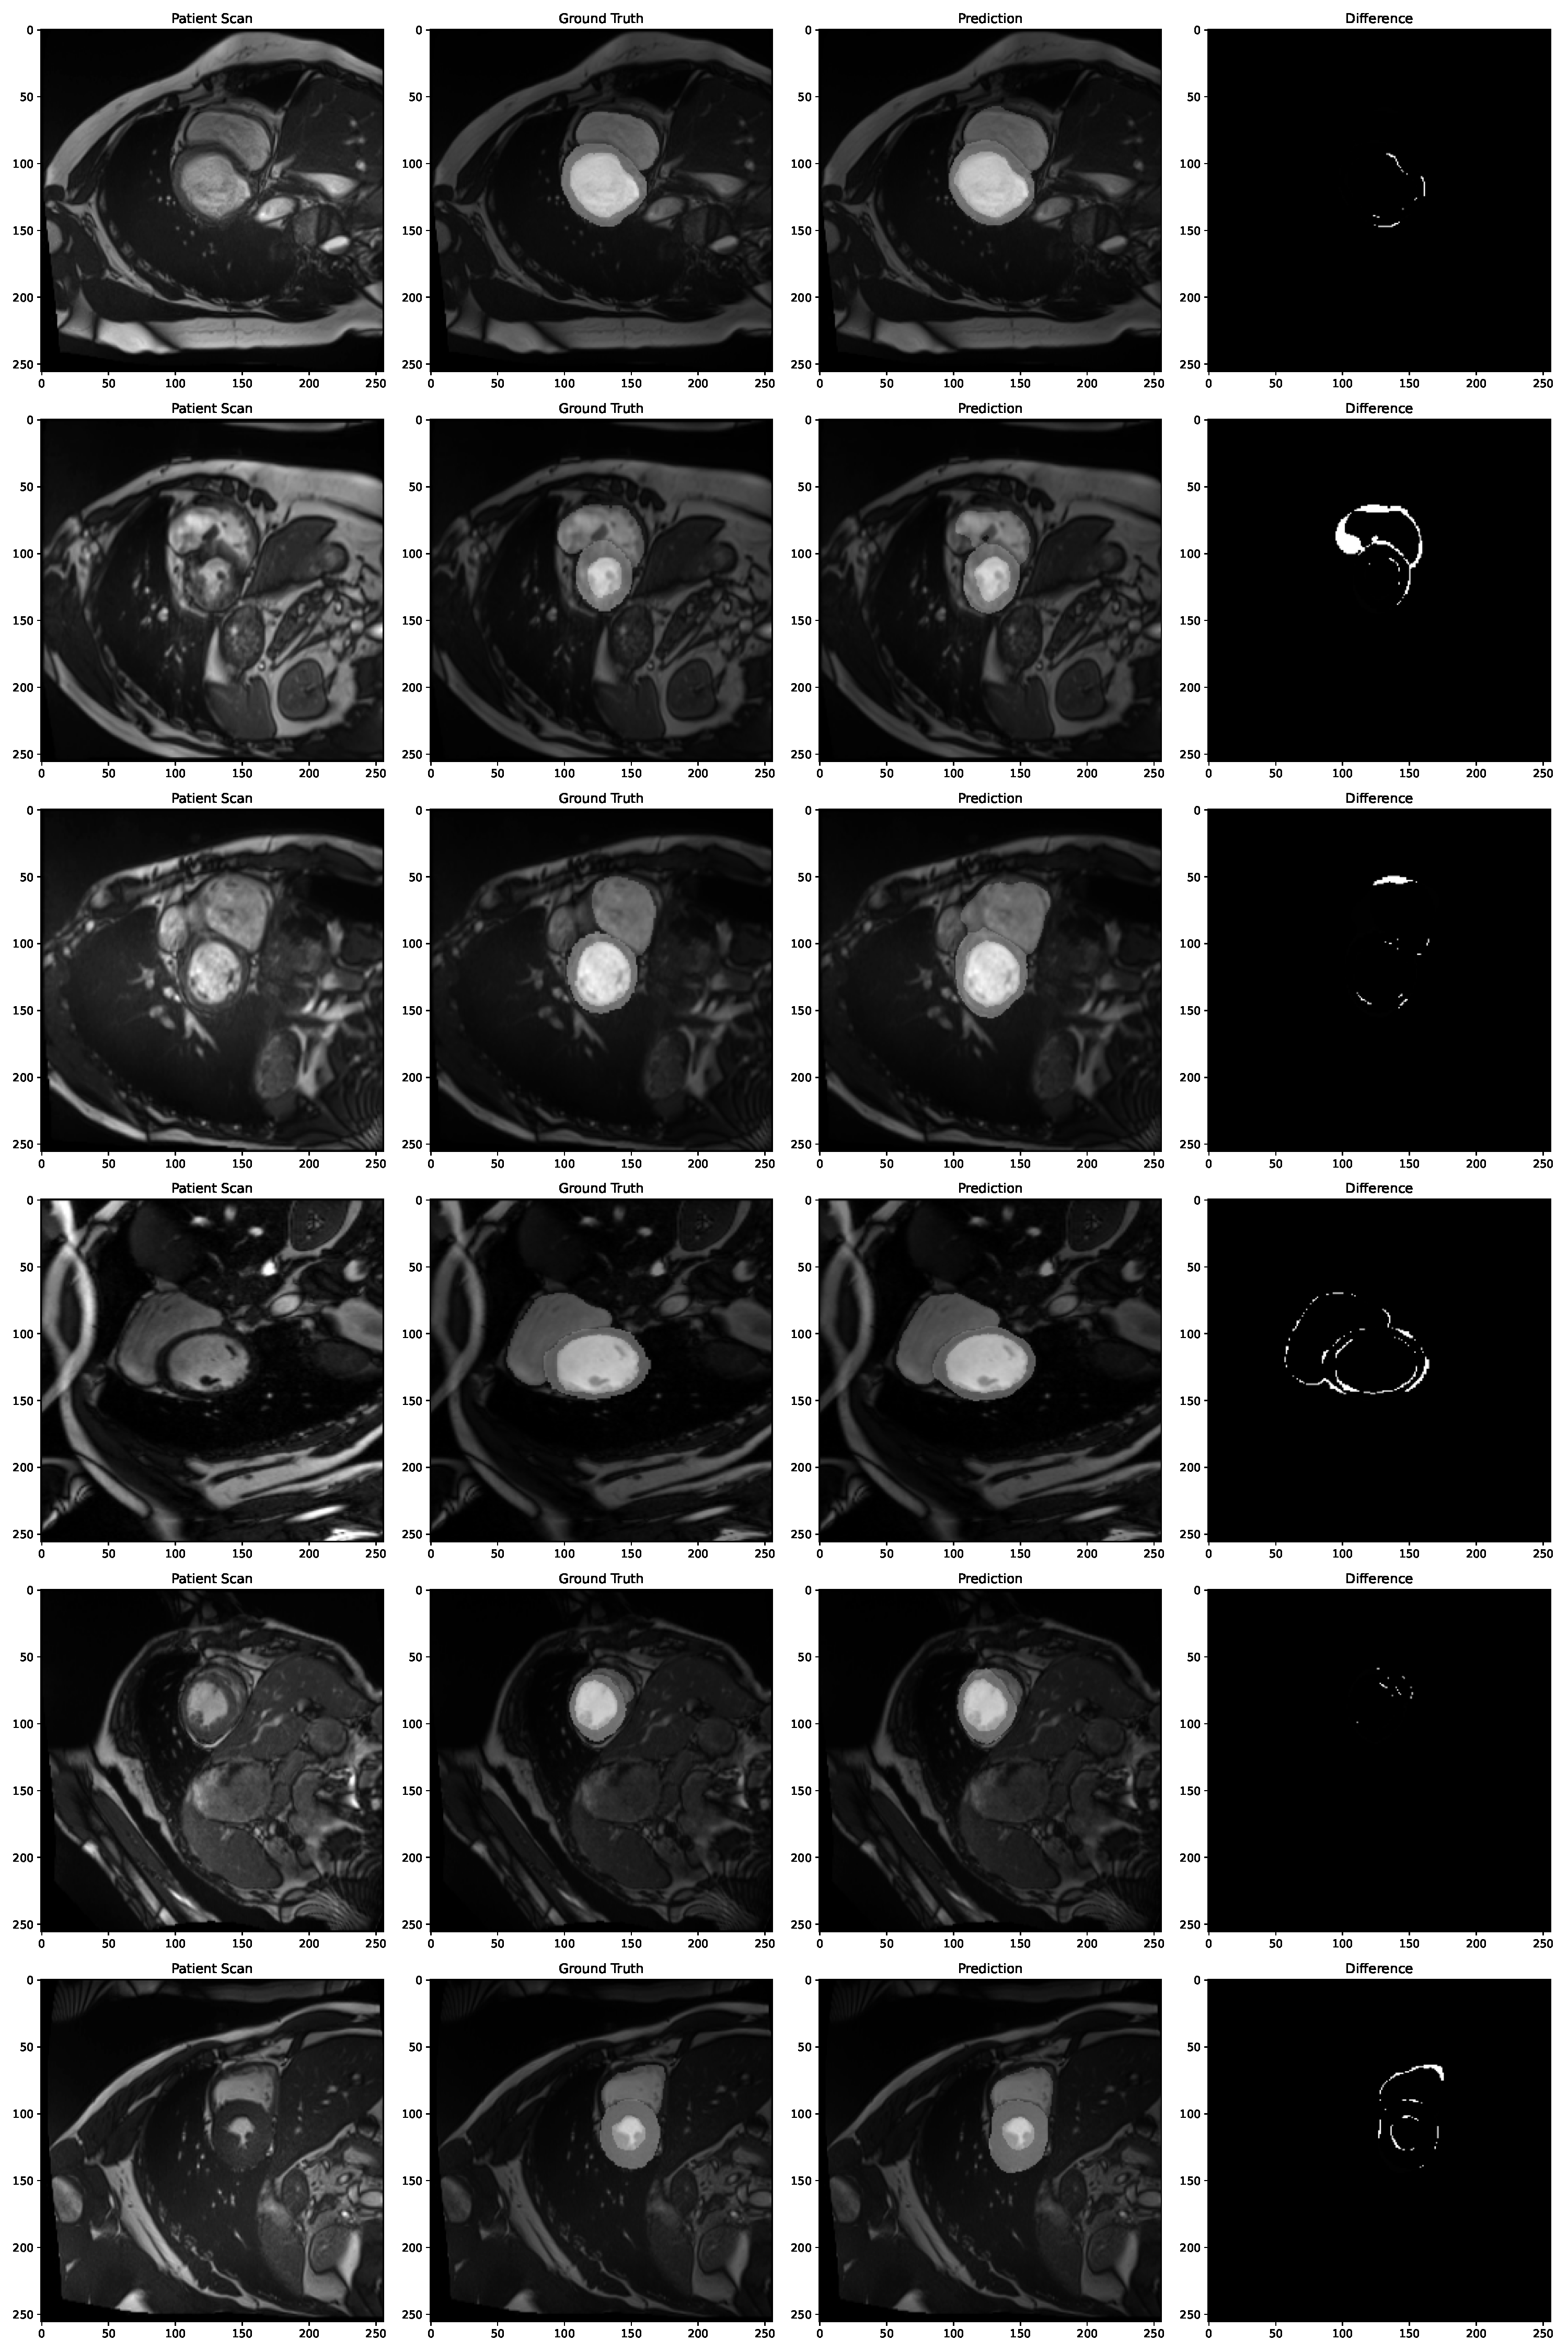
\includegraphics[width=0.8\linewidth]{figures/plot2.pdf}
    \caption{Output of the segmentation function on the validation set. 6 images out of the validation set were chosen at random. The first column corresponds to the input 2D scans, the second column to the ground truth segmentation, the third to the prediction of the CNN trained with boundary loss, and the last column illustrates the difference between the prediction and the ground truth.}
    \label{fig:plot2}
\end{figure}


\subsection{DRIVE Dataset}
\textit{Ines VATI}

\subsubsection{Experimental Design}

We also trained a model with different losses to evaluate the applicability and performance of the proposed method on the DRIVE dataset. We chose this dataset as it challenges deep learning methods due to its small size. In addition, it was not tested by the authors. The code can be found here
\url{https://github.com/InesVATI/Medical-Image-Analysis-BoundaryLoss}.

 The images for the DRIVE database were obtained from a diabetic retinopathy screening program in The Netherlands. Twenty RGB 2D images of size $(584 \times 565)$ were available along with a manual segmentation of the vasculature. Twenty other retinal images were also given for testing but their segmentation map were not made available. We thought this dataset would be interesting to evaluate and compare the method given that the vessels are thin and far less profuse than the background as can be seen in the figure \ref{ex_drive}.

We train the model on Google Colab as it provides a T4 GPU and 15 GB of RAM. However, the memory was not enough for training the network on a batch size higher than 2. Thus we downsampled the image to a size of $(256 \times 256)$.

 We also perform data augmentation by making horizontal random flips to make sure the network sees enough data. As in the article, we employed UNet as a deep learning architecture in our experiments. For the DRIVE dataset, we train a UNet network for 150 epochs with a batch size of 8\footnote{In their article, they used a batch size of 8 for the WMH dataset and 4 for the ISLE dataset. They trained on 20 epochs}. We trained a model with a UNet architecture with 4 different losses :
 \begin{itemize}
     \item with the boundary loss associated with the generalized loss: $\lcal_1 = \lcal_{GDL} + \alpha \lcal_{B}$ 
     \item with the generalized loss alone : $\lcal_2 = \lcal_{GDL}$
     \item with the cross-entropy loss alone : $\lcal_3 = \lcal_{CE}$ 
     \item with the cross-entropy associated with the boundary loss : $\lcal_4 = \lcal_{CE}+ \alpha\lcal_{B}$
 \end{itemize}
For each experiment, the weight parameter is fixed to $\alpha=0.05$. 
We chose the parameter value that gave suitable results in the experiments conducted by \cite{kervadec_boundary_2021}. They stated that even sub-optimal $\alpha$ can provide an improvement over the regional loss used alone. 

\subsubsection{Results}
\textbf{Quantitative evaluation.} During training, the dice score between ground truth and predicted segmentation map was computed on the training and validation data (see fig. \ref{fig:dsc_train_drive}). The table \ref{tab:DSC} provides the dice score on the validation data at the end of the training. The values are of the same order of magnitude as the values obtained in the article (\cite{kervadec_boundary_2021}). However, we do not observe a significant improvement over a "standalone" regional loss. To improve those results on the DRIVE dataset, we could use a scheduling strategy for $\alpha$. Indeed, \cite{kervadec_boundary_2021} noticed that increasing $\alpha$ or re-balancing the loss weights during training yields slightly better results than any constant $\alpha$. % Furthermore, the dice score computed on validation data may not be a good approximation of the performances as we used only two images in the validation dataset.

\textbf{Qualitative evaluation.} As test segmentation maps were not available, we could not compute the dice coefficient for those unseen data. However, we used test data for qualitative evaluation and computed the predicted segmentation map on random test images for each configuration. As illustrated by figure \ref{fig:tests}, the model achieves the recovery of the thin structure of the vessels. The vessels in the segmentation map computed with the model trained with $\lcal_1$ and $\lcal_4$ appear less dense than those obtained with the other models. Instead of using a fixed number of iterations to train the models, we should have used an early stopping and allowed each model to converge. 


\begin{table}[h!]
    \centering
    \begin{tabular}{c|c}
      Loss   & DSC \\
      \hline\hline
       $\lcal_{GDL} +\alpha\lcal_{B}$  & $0.788$ \\ 
       \hline
       $\lcal_{GDL}$ & $0.793$ \\
       \hline
       $\lcal_{CE}+\alpha \lcal_{B}$ & $0.763$ \\
       \hline
       $\lcal_{CE}$ & $0.798$ \\
       \hline
    \end{tabular}
    \caption{Metric after training on DRIVE validation data}
    \label{tab:DSC}
\end{table}


\begin{figure}[H]
    \centering
    \begin{subfigure}{0.45\textwidth}
        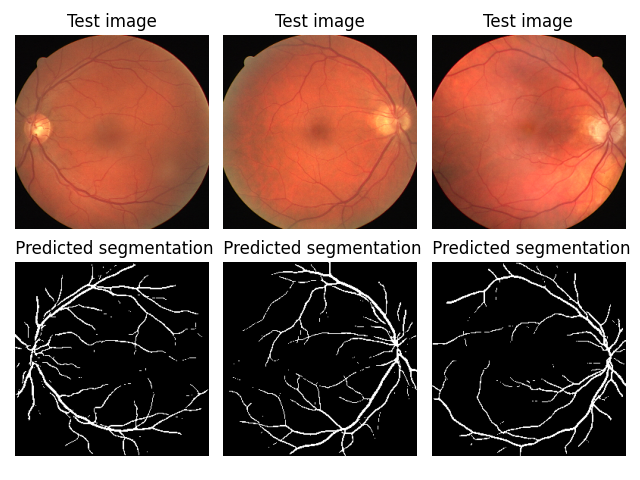
\includegraphics[width=\textwidth]{figures/result_on_test.png}
    \caption{$\lcal_1$}
    \end{subfigure}
    \begin{subfigure}{0.45\textwidth}
        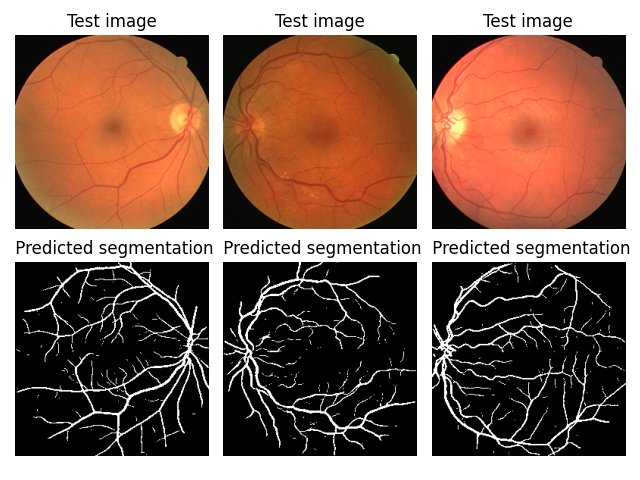
\includegraphics[width=\textwidth]{figures/results_on_testGDL.png}
    \caption{$\lcal_2$}
    \end{subfigure}
    \begin{subfigure}{0.45\textwidth}
        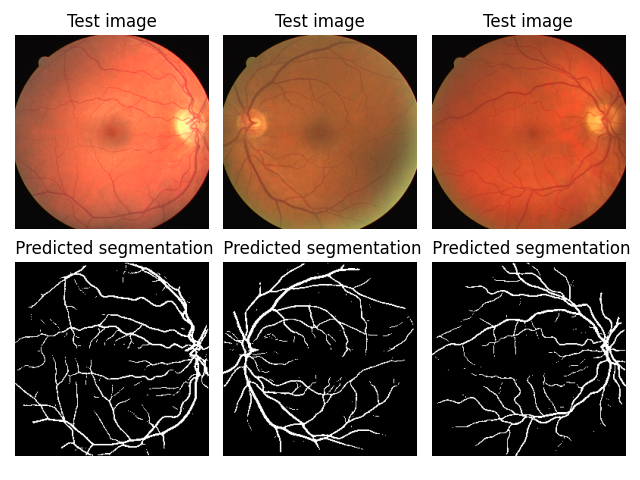
\includegraphics[width=\textwidth]{figures/results_on_testCE.png}
    \caption{$\lcal_3$}
    \end{subfigure}
    \begin{subfigure}{0.45\textwidth}
        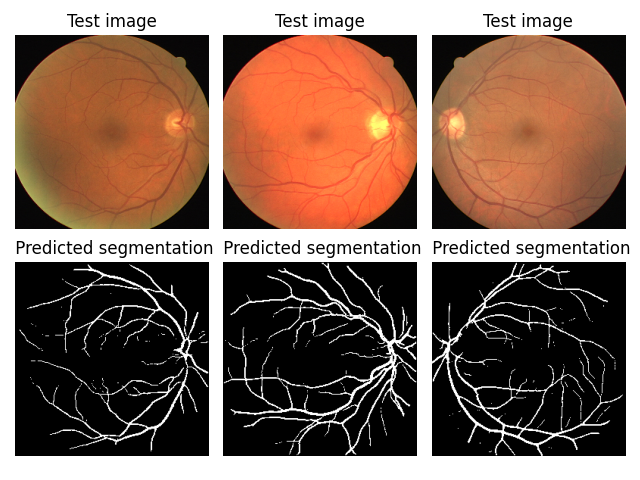
\includegraphics[width=\textwidth]{figures/results_on_testCEwBL.png}
    \caption{$\lcal_4$}
    \end{subfigure}
    \caption{Evaluation of the trained model on test images}
    \label{fig:tests}
\end{figure}

% \section{Discussion??}
% \textit{Ines Vati} and \textit{Mahmoud Hegazy}




\medskip

\bibliographystyle{plainnat}
\bibliography{ref}

\clearpage
\appendix
\appendixpage % ajoute par defaut le titre "Appendices" au dessus de la première annexe
\section{DRIVE Database}

\begin{figure}[h!]
    \centering
    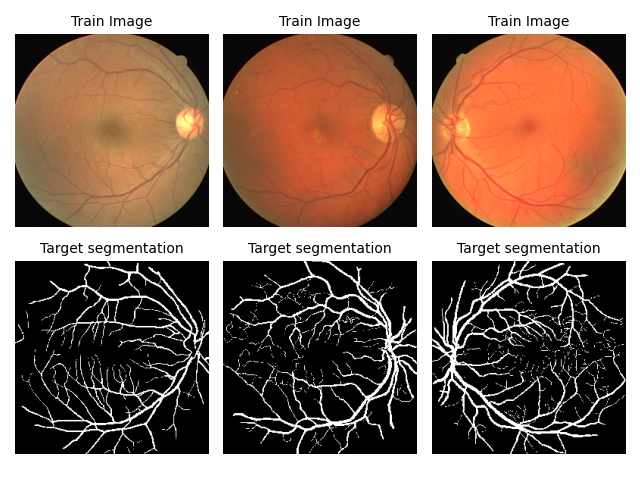
\includegraphics[width=\textwidth]{figures/ex_drive.png}
    \caption{Examples of DRIVE database}
    \label{ex_drive}
\end{figure}
 
\section{Learning curves for DRIVE dataset}

\begin{figure}[H]
    \centering
    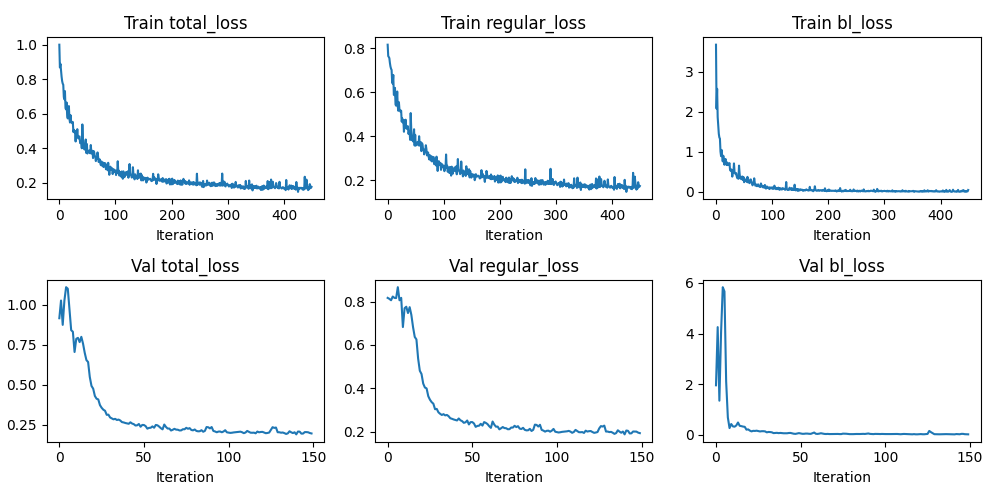
\includegraphics[width=\textwidth]{figures/learning_curves.png}
    \caption{Loss evolution during training of DRIVE dataset with $\lcal_1$. The "regular\_loss" is $\lcal_{GDL}$}
    \label{fig:learn_curves_drive}
\end{figure}

\begin{figure}[H]
    \centering
    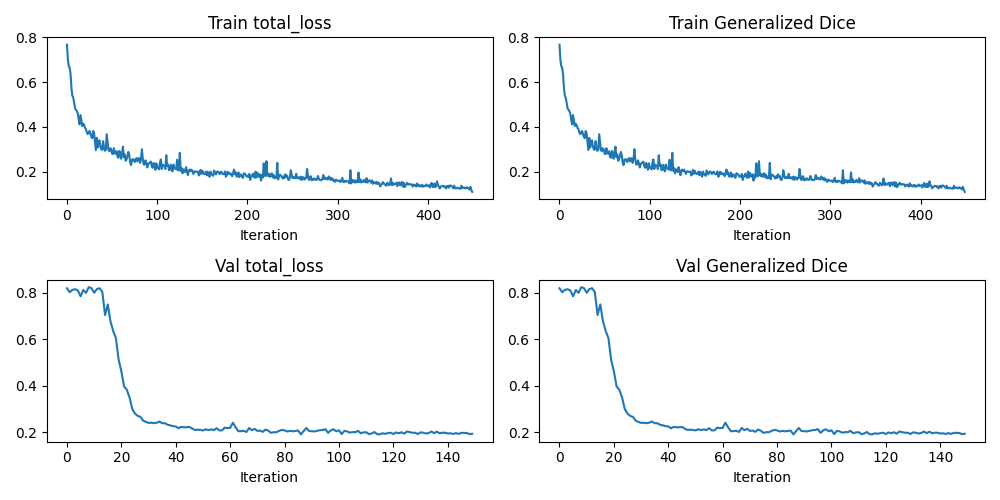
\includegraphics[width=\textwidth]{figures/GDL_learning_curves.png}
    \caption{Loss evolution during training of DRIVE dataset with $\lcal_2$ (without boundary loss)}
    \label{fig:learn_curve_drive_l2}
\end{figure}

\begin{figure}[H]
    \centering
    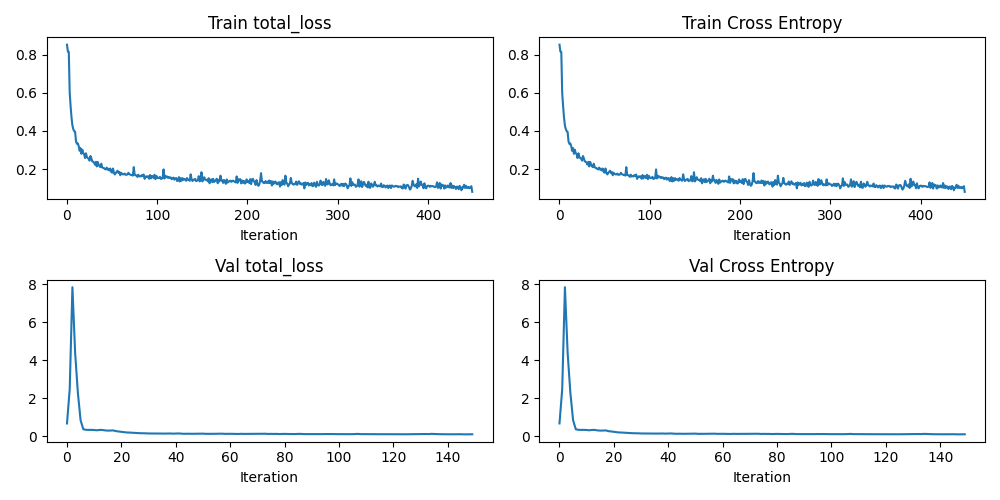
\includegraphics[width=\textwidth]{figures/CE_learning_curves.png}
    \caption{Loss evolution during training of DRIVE dataset with $\lcal_3$}
    \label{fig:learn_drive_l3}
\end{figure}

\begin{figure}[H]
    \centering
    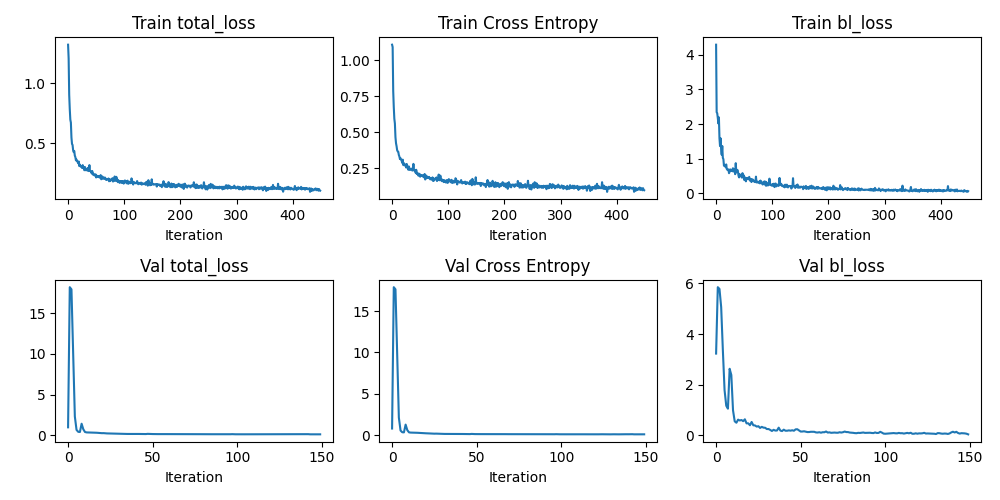
\includegraphics[width=\textwidth]{figures/CEwBL_learning_curves.png}
    \caption{Loss evolution during training of DRIVE dataset with $\lcal_4$}
    \label{fig:learn_drive_l4}
\end{figure}

\section{Dice score on DRIVE dataset}

\begin{figure}[h!]
    \centering
    \begin{subfigure}{0.45\textwidth}
        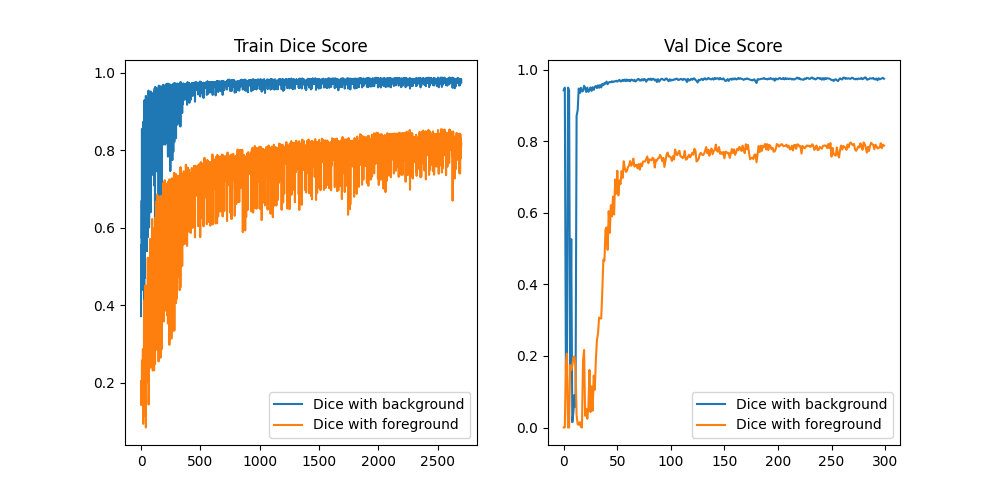
\includegraphics[width=\textwidth]{figures/dice_coeff_training.png}
        \caption{$\lcal_1$}
    \end{subfigure}
    \begin{subfigure}{0.45\textwidth}
        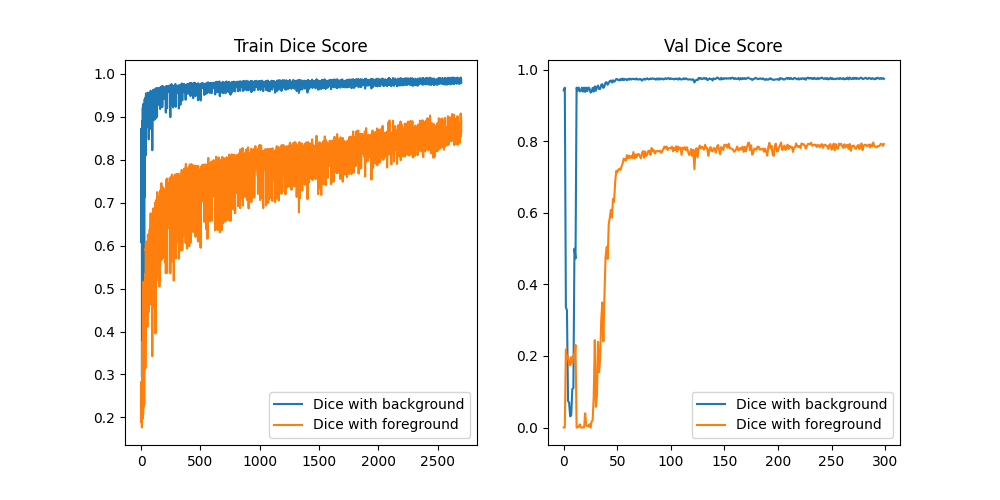
\includegraphics[width=\textwidth]{figures/GDL_dice_coeff_training.png}
        \caption{$\lcal_2$}
    \end{subfigure}
    \begin{subfigure}{0.45\textwidth}
        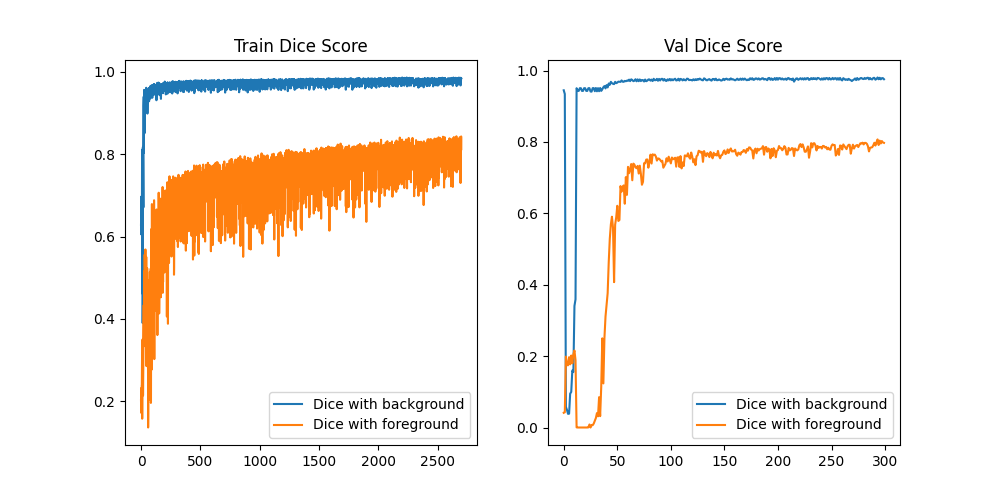
\includegraphics[width=\textwidth]{figures/CE_dice_coeff_training.png}
        \caption{$\lcal_{3}$}
    \end{subfigure}
    \begin{subfigure}{0.45\textwidth}
        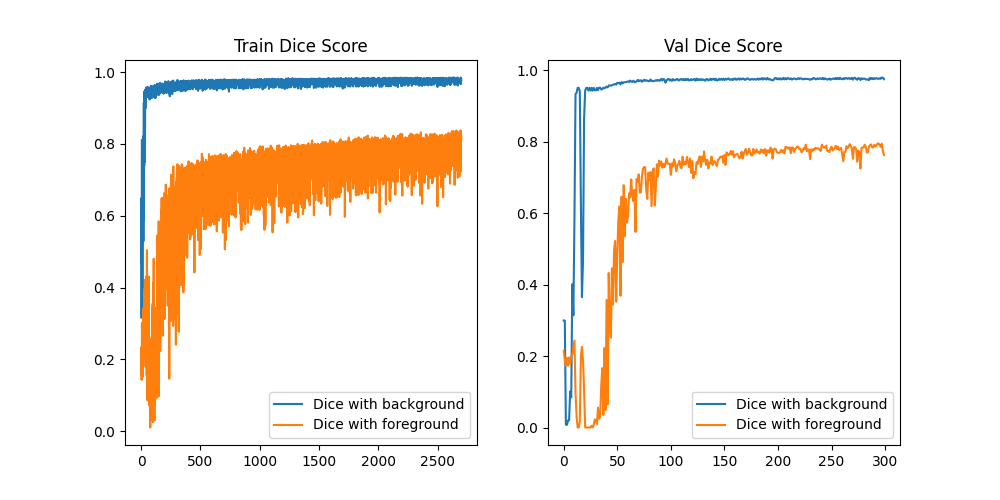
\includegraphics[width=\textwidth]{figures/CEwBL_dice_coeff_training.png}
        \caption{$\lcal_{4}$}
    \end{subfigure}
    \caption{Evolution of the dice score during training on DRIVE dataset} The dice score for the foreground and background are plotted for the training and validation dataset. $\lcal_{1}$, $\lcal_2$ and $\lcal_3$ are the different losses evaluated during the experiments described above. $\lcal_3$ is the "baseline" loss. In our case, it is the cross-entropy loss function.
    \label{fig:dsc_train_drive}
\end{figure}

\end{document}
